\documentclass[tikz,border={18pt 10pt 10pt 8pt}]{standalone}
\usepackage[T1]{fontenc}
\usepackage[scaled=0.92]{helvet}
\renewcommand{\familydefault}{\sfdefault}
\usepackage{amsmath,amssymb}
\usetikzlibrary{arrows.meta, positioning, calc, backgrounds}

\definecolor{cPrimary}{RGB}{0, 102, 180}
\definecolor{cWarning}{RGB}{200, 110, 10}
\definecolor{cDanger}{RGB}{209, 34, 57}
\definecolor{cSafe}{RGB}{34, 139, 34}

% Substation line colors
\definecolor{cFuji}{RGB}{0, 90, 160}
\definecolor{cHatano}{RGB}{120, 50, 160}
\definecolor{cTama}{RGB}{20, 140, 120}
\definecolor{cKoga}{RGB}{190, 95, 15}

\begin{document}
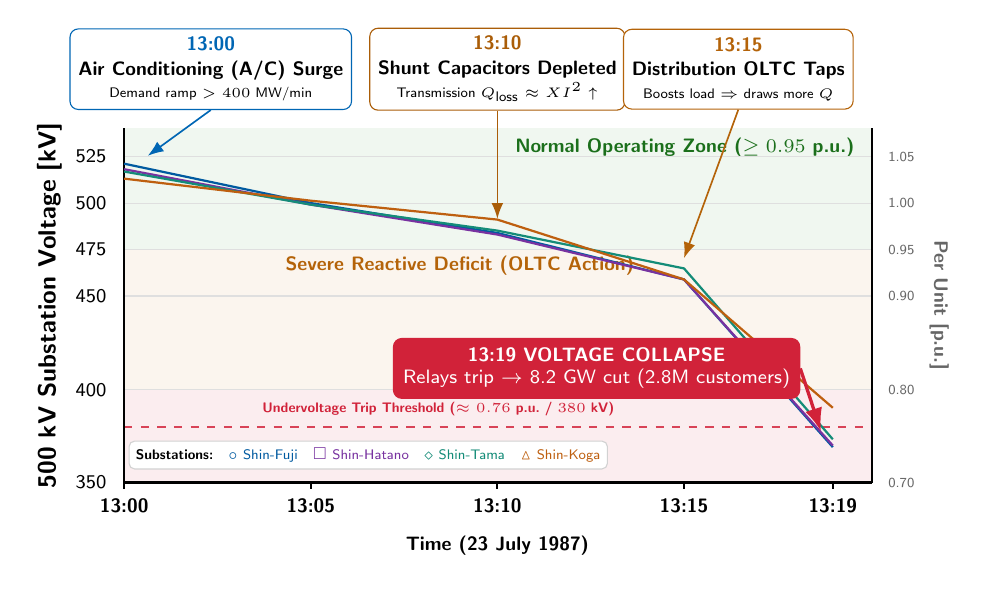
\begin{tikzpicture}[>=Latex, font=\sffamily]

    % Dimensions: x from 0 to 9.5 cm, y from 0 to 4.5 cm
    % Time: 13:00 (x=0) to 13:19 (x=9.0)
    
    % Background bands
    % Safe zone: 475 to 540 kV (y=2.96 to 4.5)
    \fill[cSafe!7] (0, 2.96) rectangle (9.5, 4.5);
    % Warning zone: 400 to 475 kV (y=1.18 to 2.96)
    \fill[cWarning!7] (0, 1.18) rectangle (9.5, 2.96);
    % Collapse zone: 350 to 400 kV (y=0 to 1.18)
    \fill[cDanger!8] (0, 0) rectangle (9.5, 1.18);
    
    % Zone labels on right inside plot
    \node[anchor=east, font=\scriptsize\bfseries, text=cSafe!80!black] at (9.4, 4.25) {Normal Operating Zone ($\ge 0.95\text{ p.u.}$)};
    \node[anchor=east, font=\scriptsize\bfseries, text=cWarning!90!black] at (6.6, 2.75) {Severe Reactive Deficit (OLTC Action)};
    \node[anchor=west, font=\scriptsize\bfseries, text=cDanger!90!black] at (0.2, 0.35) {Collapse Zone};

    % Threshold line (380 kV / 0.76 pu -> y = 0.71)
    \draw[thick, dashed, cDanger!85] (0, 0.71) -- (9.5, 0.71) 
        node[pos=0.42, above, font=\tiny\bfseries, text=cDanger] {Undervoltage Trip Threshold ($\approx 0.76\text{ p.u.}$ / $380\text{ kV}$)};

    % Grid lines (horizontal)
    \foreach \kV/\y/\pu in {350/0.0/0.70, 400/1.18/0.80, 450/2.37/0.90, 475/2.96/0.95, 500/3.55/1.00, 525/4.14/1.05} {
        \draw[gray!25, thin] (0, \y) -- (9.5, \y);
        \node[anchor=east, font=\scriptsize] at (-0.1, \y) {\kV};
        \node[anchor=west, font=\tiny, text=gray!80!black] at (9.58, \y) {\pu};
    }
    
    % Y axis labels
    \node[rotate=90, font=\small\bfseries] at (-0.95, 2.25) {500 kV Substation Voltage [kV]};
    \node[rotate=-90, font=\scriptsize\bfseries, text=gray!80!black] at (10.35, 2.25) {Per Unit [p.u.]};

    % Axes
    \draw[thick] (0, 0) -- (9.5, 0);
    \draw[thick] (0, 0) -- (0, 4.5);
    \draw[thick] (9.5, 0) -- (9.5, 4.5);

    % X ticks and labels
    \foreach \t/\x in {13:00/0, 13:05/2.37, 13:10/4.74, 13:15/7.11, 13:19/9.0} {
        \draw[thick] (\x, 0) -- (\x, -0.08);
        \node[below, font=\scriptsize\bfseries] at (\x, -0.08) {\t};
    }
    \node[below, font=\scriptsize\bfseries] at (4.74, -0.55) {Time (23 July 1987)};

    % Substation Curves:
    % 1. Shin-Fuji
    \draw[thick, cFuji, mark=o, mark size=1.8pt, mark options={fill=white, draw=cFuji}] 
        (0, 4.05) -- (2.37, 3.55) -- (4.74, 3.17) -- (7.11, 2.58) -- (9.0, 0.45);

    % 2. Shin-Hatano
    \draw[thick, cHatano, mark=square*, mark size=1.4pt, mark options={fill=white, draw=cHatano}] 
        (0, 3.98) -- (2.37, 3.53) -- (4.74, 3.15) -- (7.11, 2.58) -- (9.0, 0.47);

    % 3. Shin-Tama
    \draw[thick, cTama, mark=diamond*, mark size=1.7pt, mark options={fill=white, draw=cTama}] 
        (0, 3.95) -- (2.37, 3.53) -- (4.74, 3.20) -- (7.11, 2.72) -- (9.0, 0.55);

    % 4. Shin-Koga
    \draw[thick, cKoga, mark=triangle*, mark size=1.7pt, mark options={fill=white, draw=cKoga}] 
        (0, 3.86) -- (2.37, 3.58) -- (4.74, 3.34) -- (7.11, 2.58) -- (9.0, 0.95);

    % Milestone annotations above the plot
    % 13:00 Callout
    \node[draw=cPrimary, fill=white, rounded corners=3pt, font=\scriptsize, align=center, inner sep=3pt] (noteA) at (1.1, 5.25) {
        \textbf{\color{cPrimary}13:00}\\[1pt]
        \textbf{Air Conditioning (A/C) Surge}\\
        \tiny Demand ramp $>400\text{ MW/min}$
    };
    \draw[->, semithick, cPrimary] (noteA.south) -- (0.3, 4.15);

    % 13:10 Callout
    \node[draw=cWarning!85!black, fill=white, rounded corners=3pt, font=\scriptsize, align=center, inner sep=3pt] (noteB) at (4.74, 5.25) {
        \textbf{\color{cWarning!85!black}13:10}\\[1pt]
        \textbf{Shunt Capacitors Depleted}\\
        \tiny Transmission $Q_{\text{loss}} \approx X I^2 \uparrow$
    };
    \draw[->, semithick, cWarning!85!black] (noteB.south) -- (4.74, 3.35);

    % 13:15 Callout
    \node[draw=cWarning!90!black, fill=white, rounded corners=3pt, font=\scriptsize, align=center, inner sep=3pt] (noteC) at (7.8, 5.25) {
        \textbf{\color{cWarning!90!black}13:15}\\[1pt]
        \textbf{Distribution OLTC Taps}\\
        \tiny Boosts load $\Rightarrow$ draws more $Q$
    };
    \draw[->, semithick, cWarning!90!black] (noteC.south) -- (7.11, 2.85);

    % 13:19 Collapse Callout
    \node[draw=cDanger, fill=cDanger, text=white, rounded corners=3pt, font=\scriptsize\bfseries, align=center, inner sep=3.5pt] (noteD) at (6.0, 1.45) {
        13:19 VOLTAGE COLLAPSE\\
        \scriptsize\textmd{Relays trip $\to$ 8.2 GW cut (2.8M customers)}
    };
    \draw[->, very thick, cDanger] (noteD.east) -- (8.85, 0.65);

    % Substation Legend
    \node[draw=gray!35, fill=white, rounded corners=2pt, inner sep=2.5pt, font=\tiny] at (3.1, 0.35) {
        \textbf{Substations:}\quad
        {\color{cFuji}$\circ$ Shin-Fuji}\quad
        {\color{cHatano}$\square$ Shin-Hatano}\quad
        {\color{cTama}$\diamond$ Shin-Tama}\quad
        {\color{cKoga}$\vartriangle$ Shin-Koga}
    };

\end{tikzpicture}
\end{document}
